\documentclass{report}
% Change "article" to "report" to get rid of page number on title page
\usepackage{amsmath,amsfonts,amsthm,amssymb}
\usepackage{setspace}
\usepackage{Tabbing}
\usepackage{fancyhdr}
\usepackage{lastpage}
\usepackage{extramarks}
\usepackage{chngpage}
\usepackage{soul,color}
\usepackage{listings}
\usepackage{enumerate}
\usepackage{graphicx,float,wrapfig}
\usepackage{pifont}
\usepackage{graphicx}
\usepackage[english]{babel}
\usepackage{tikz}
\usepackage[]{algorithm2e}
% In case you need to adjust margins:
\topmargin=-0.45in      %
\evensidemargin=0in     %
\oddsidemargin=0in      %
\textwidth=6.5in        %
\textheight=9.0in       %
\headsep=0.25in         %

\title{Assignment 1 - Comp 652 - Machine Learning}

% Homework Specific Information
\newcommand{\hmwkTitle}{Assignment 3}                     % Adjust this
\newcommand{\hmwkDueDate}{Tuesday, March 31 2015}                           % Adjust this
\newcommand{\hmwkClass}{COMP 652}


\newcommand{\hmwkClassInstructor}{Dr. Doina Precup}
\newcommand{\hmwkAuthorName}{Geoffrey Stanley}
\newcommand{\hmwkAuthorNumber}{260645907}
\newcommand{\Pp}{\mathbb{P}}
\newcommand{\Ev}{\mathbb{E}}
\newcommand{\cov}{\text{Cov}}
\newcommand{\Z}{\mathbb{Z}}
\newcommand{\R}{\mathbb{R}}
\newcommand{\dd}{\, \mathrm{d}}

% Setup the header and footer
\pagestyle{fancy}                                                       %
\lhead{\hmwkAuthorName}                              %
\chead{}
\rhead{\hmwkClass: \hmwkTitle}                                          %

\lfoot{}
\cfoot{}                                                                %
\rfoot{Page\ \thepage\ of\ \pageref{LastPage}}                          %
\renewcommand\headrulewidth{0.4pt}                                      %
\renewcommand\footrulewidth{0.4pt}                                      %

% This is used to trace down (pin point) problems
% in latexing a document:
%\tracingall
\definecolor{mygreen}{rgb}{0,0.6,0}
\lstset{commentstyle=\color{mygreen}, frame=single,  language=R, showspaces=false, showstringspaces=false}

%%%%%%%%%%%%%%%%%%%%%%%%%%%%%%%%%%%%%%%%%%%%%%%%%%%%%%%%%%%%%
% Make title
\title{\vspace{2in}\textmd{\textbf{\hmwkClass:\ \hmwkTitle}}\\
\normalsize\vspace{0.1in}\small{Due\ on\ \hmwkDueDate}\\
\vspace{0.1in}\large{\textit{Presented to \hmwkClassInstructor}}\vspace{3in}}
\date{}
\author{\textbf{\hmwkAuthorName}\\
    \textbf{Student ID: \hmwkAuthorNumber}}
%%%%%%%%%%%%%%%%%%%%%%%%%%%%%%%%%%%%%%%%%%%%%%%%%%%%%%%%%%%%%

\begin{document}
\maketitle
\section*{Question 1}
\subsection*{A)}
In the 4-neighbor spin glass model the maximal cliques were the edges between
each pixel. In an 8-neighbor spin glass model the maximal cliques become
clusters of 4 pixels. As such, parametization for a 4 neighbor spin glass model
will be as follows:

\begin{center}
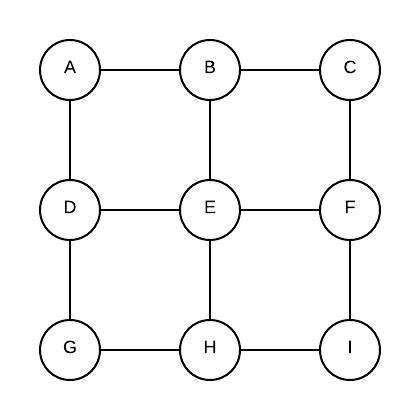
\includegraphics[width=125pt, keepaspectratio=true]{ising_model_4n.jpg}\\
\end{center}
\begin{equation}
  P(E) = \psi (B,E) \psi (D,E) \psi (E,F) \psi (E,H)
\end{equation}
While the parameters for an 8 neighbor spin glass model will be as such:
\begin{center}
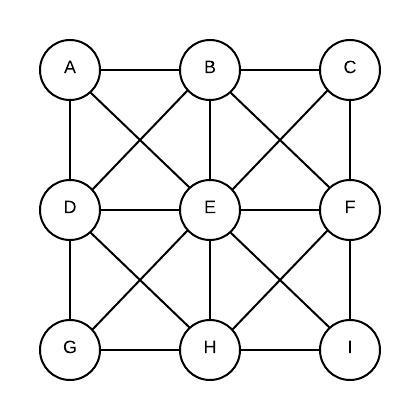
\includegraphics[width=125pt, keepaspectratio=true]{ising_model_8n.jpg}\\
\end{center}
\begin{equation}
  P(E) = \psi (A,B,D,E) \psi (B,C,E,F) \psi (D,E,G,H) \psi (E,F,H,I)
\end{equation}

\subsection*{B)}
The advantages and disadvantages would be related to a trade off between
model precision and computation time.\\

Given a 4 neighbor model computation time will be smaller given 20 fewer edge
energy to be computed. However, the is at the expense of model accuracy. With
the 8 neighbor model more data will be used to infer the value a pixel and
as such would be more flexible. Which should improve the models accuracy.\\

In particular, with an 8 neighbor model would be able to model an image that contain
circular shapes or curved lines.
\subsection*{C)}

\section*{Question 2}
\begin{center}
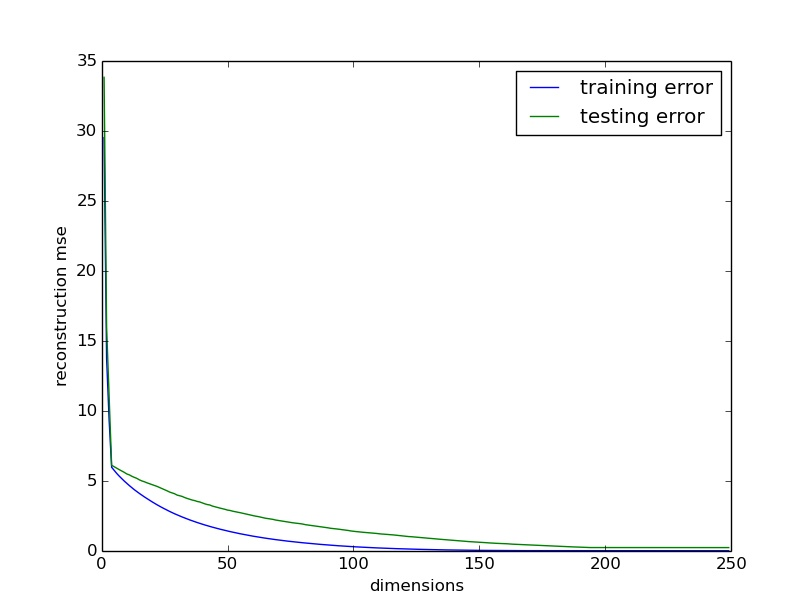
\includegraphics[width=250pt, keepaspectratio=true]{reconstruction_error.jpg}\\
\end{center}
As dimensions are reduced from 250 the reconstruction error is initially quite
small but becomes more important as dimensions approach 0. The
shoulder of the reconstruction error line is at a dimension of approximately 25.\\

From this, we can conclude that given this input space we can use PCA to
reduce dimensionality of the data to 25 in order to make computation more manageable
without losing very much granularity in the feature data.
\section*{Question 3}
\subsection*{A)}
As with standard Hidden Markov Models, Coupled Hidden Markov models will
have three categories of parameters. These are the initial probabilities, the
transition probabilites and the emission probabilities. Given the system
depicted in Figure 1 of assignment 3:\\

Initial Probabilities:
\begin{equation}
  P(s0)
\end{equation}
\begin{equation}
  P(u0)
\end{equation}\\

Transition Probabilities:
\begin{equation}
  P(s_i | s_{i-1}, u_{i-1})
\end{equation}
\begin{equation}
  P(u_i | u_{i-1}, s_{i-1})
\end{equation}\\

Emission Probabilities:
\begin{equation}
  P(y_i | s_i)
\end{equation}
\begin{equation}
  P(z_i | u_i)
\end{equation}

\subsection*{B)}
In order to compute the joint probability of a sequence of observations a
forward algorithm will need to be derived.

\begin{equation}
  \begin{aligned}
  \alpha_t(s_t, u_t) & = P(s_t, u_t, y_{0:T}, x_{0:T})\\
   & = \sum_{t = 1}^T p(s_t, s_{t-1}, u_t, u_{t-1}, y_{1:T}, x_{1:T})\\
   & = \sum_{t = 1}^T p(y_t | s_t) p(x_t | u_t) p(s_t | s_{t-1}, u_{t-1}) p(u_t | s_{t-1}, u_{t-1}) p(s_{t-1}, u_{t-1}, y_{1:T-1}, x_{1:T-1})\\
   & = \sum_{t = 1}^T p(y_t | s_t) p(x_t | u_t) p(s_t | s_{t-1}, u_{t-1}) p(u_t | s_{t-1}, u_{t-1}) \alpha_{t-1}(y_{t-1}, x_{t-1})
  \end{aligned}
\end{equation}
Because the equation listed above does not contain the initial probability we
need to compute it seperately:
\begin{equation}
  \alpha_0 (s_0, u_0) = p(y_0, z_0, s_0, u_0) = p(s_0) p(y_0 | s_0) p(u_0) p(z_0 | u_0)
\end{equation}
Summing the equations above we obtain the joint probability:
\begin{equation}
  p(y_0, z_0, y_1, z_1, ... , y_T, z_T) = \sum_{i=0}^T \alpha_i(s_i, u_i)
\end{equation}

\subsection*{C)}
The forward-backward algorithm is equal to the product between the forward and the
backward algorithm. In the previous question I derived the forward algorithm. So,
what is remaining is to derive the backward algorithm:
\begin{equation}
  \begin{aligned}
    \beta_t(s_t, u_t) & = p(y_{t+1:n} | s_t, u_t) p(z_{t+1:n} | s_t, u_t)\\
    & = \sum_{k=0}^{T-1} p(y_{t+1:n}, z_{t+1:n}, s_{t+1}, u_{t+1} | s_t, u_t)\\
    & = \sum_{k=0}^{T-1} p(y_{t+2:n} | s_{t+1}, u_{t+1}) p(z_{t+2:n} | s_{t+1}, u_{t+1}) p(y_{t+1} | s_{t+1}) p(z_{t+1} | u_{t+1}) p(s_{t+1} | s_t, u_t) p(u_{t+1} | s_t, u_t)\\
    & = \sum_{k=0}^{T-1} \beta_{t+1}(s_{t+1}, u_{t+1}) p(y_{t+1} | s_{t+1}) p(z_{t+1} | u_{t+1}) p(s_{t+1} | s_t, u_t) p(u_{t+1} | s_t, u_t)
  \end{aligned}
\end{equation}
The probability at time T will be equal to 1 :
\begin{equation}
  \beta_T (s_T, u_T) = 1
\end{equation}
Summing the equations above we obtain te backward algorithm:
\begin{equation}
p(y_{t+1:n} | s_t, u_t) p(z_{t+1:n} | s_t, u_t) = \sum_{i=0}^{T} \beta_i(s_i, u_i)
\end{equation}
We can now derive the forward-backward algorithm as the product between the forward
and the backward algorithm:
\begin{equation}
p(s_t, u_t | y_{0:T}, x_{0:T}) = \left(\sum_{i=0}^T \alpha_i(s_i, u_i)\right)\left( \sum_{i=0}^{T} \beta_i(s_i, u_i)\right)
\end{equation}

\subsection*{D)}
The transition probabilities as well as the inference algorithms used will be
conditional on whether $t\mod{k}=0$. More precisely, for transition probabilities:

\begin{equation}
  \left\{
  \begin{array}{l l}
    P(s_i | s_{i-1}, u_{i-1}) & \quad \text{if } i \mod k = 0 \\
    P(s_i | s_{i-1}) & \quad \text{otherwise}

  \end{array} \right.
\end{equation}

\begin{equation}
  \left\{
  \begin{array}{l l}
    P(u_i | u_{i-1}, s_{i-1}) & \quad \text{if } i \mod k = 0 \\
    P(u_i | u_{i-1}) & \quad \text{otherwise}

  \end{array} \right.
\end{equation}\\
And the computation for the inference algorithms will be similar. For the forward
algorithm:
\begin{equation}
  \left\{
  \begin{array}{l l}
  \sum_{t = 1}^T p(y_t | s_t) p(x_t | u_t) p(s_t | s_{t-1}, u_{t-1}) p(u_t | s_{t-1}, u_{t-1}) \alpha_{t-1}(y_{t-1}, x_{t-1}) & \quad \text{if } t \mod k = 0 \\
  \sum_{t = 1}^T p(y_t | s_t) p(x_t | u_t) p(s_t | s_{t-1}) p(u_t | u_{t-1}) \alpha_{t-1}(y_{t-1}, x_{t-1}) & \quad \text{otherwise}

  \end{array} \right.
\end{equation}\\
And for the backward algorithm:
\begin{equation}
  \left\{
  \begin{array}{l l}
  \sum_{t=0}^{T-1} \beta_{t+1}(s_{t+1}, u_{t+1}) p(y_{t+1} | s_{t+1}) p(z_{t+1} | u_{t+1}) p(s_{t+1} | s_t, u_t) p(u_{t+1} | s_t, u_t) & \quad \text{if } i \mod k = 0 \\
  \sum_{t=0}^{T-1} \beta_{t+1}(s_{t+1}, u_{t+1}) p(y_{t+1} | s_{t+1}) p(z_{t+1} | u_{t+1}) p(s_{t+1} | s_t) p(u_{t+1} | u_t) & \quad \text{otherwise}

  \end{array} \right.
\end{equation}\\
\subsection*{E)}
The object of the learning algorithm should be to find the $K$ whose joint probability
is the greatest. As such, for each $K$ in the the range $0$ to $n$ the joint probability
will have to be calculated. Once this is done, the $K$ whose joint probability is the
greatest should be used as the most accurate model.

\end{document}
